\documentclass{article}
\usepackage{graphicx}
\usepackage{hyperref}
\usepackage{float}
\usepackage{multicol}

\title{Práctica 1}

\author{Algoritmos de Ordenamiento Parte 1}

\begin{document}
	
	\maketitle
	
	\section{Objetivo}
	El estudiante identificará la estructura de los algoritmos de ordenamiento InsertionSort, SelectionSort y HeapSort.
	
	\section{Desarrollo}
		
		\subsection{Ejercicio 1}
		
		
			\subsubsection{utilidades.h}
			
			El archivo de \verb*|utilidades.h| contiene prototipos de funciones auxiliares para la ejecución de la biblioteca \verb*|ordenamientos.c|. Los prototipos de las funciones, son los siguientes:
			
			\begin{itemize}
				\item swap
				\item printArray
				\item printSubArray
			\end{itemize}
			
			\subsubsection{utilidades.c}
			
			El archivo de \verb*|utilidades.c| contiene la declaración de las 3 funciones auxiliares que servirán a \verb*|ordenamientos.c| principalmente para el \emph{output} grafico del resultado de la ejecución de los algoritmos de ordenamiento.\\
			
			Las funciones incluidas, son las siguientes:
			
			\begin{itemize}
				
				\item swap()
				
				La función \emph{swap} es de tipo \emph{void} (lo que significa que no devuelve ningún tipo de dato) y utiliza dos apuntadores como argumentos que son \emph{a} y \emph{b}. Dentro de la función se utiliza una variable \emph{t} para depositar el valor en \emph{a}, después, se asigna el valor en \emph{b} al valor en \emph{a} y por ultimo se transmite el valor depositado en la variable temporal \emph{t} a donde apunta \emph{b}.
				
				\item printArray()
				
				La función \emph{printArray}, toma como argumento un arreglo de enteros \emph{arr} y la longitud de ese arreglo con una variable entera \emph{size}. Después declara una variable entera \emph{i} para efectos del \emph{for-loop} que ira imprimiendo cada uno de los valores dentro del arreglo.
				
				Al finalizar la función imprime un salto de linea.
				
				\item printSubArray()
				
				La función \emph{printSubArray} toma 3 argumentos que son un arreglo de enteros \emph{arr} y dos variables enteras, \emph{low} y \emph{high}. Después, ya dentro de la función, se declara una variable entera \emph{i} para que funcione como contador dentro del \emph{for-loop} y se imprime la leyenda \emph{"Sub array:"}antes de comenzar a imprimir el arreglo.
				
				Al momento de iniciar el \emph{for-loop} el valor en \emph{low} se asigna a la variable \emph{i} y comenzara a iterar sumando 1 en cada ciclo hasta alcanzar un valor menor o igual al existente en la variable \emph{high}, en cada ciclo se imprime el valor del arreglo a partir del indice contenido en \emph{low} y termina con el valor en el indice \emph{high}.
				
				Al finalizar la función, imprime un salto de linea.
				
			\end{itemize}
			
			
			\subsubsection{ordenamientos.h}
			
			El archivo ordenamientos.h contiene el prototipo de las funciones que se describen en el archivo \verb*|ordenamientos.c|\\
			
			Contiene 5 prototipos que son:
			
			\begin{itemize}
				\item selectionSort
				\item insertionSort
				\item HeapSort
				\item BuildHeap
				\item Heapify
			\end{itemize}
			
			\subsubsection{ordenamientos.c}
			
			Este archivo contiene el código de cada una de las funciones declaradas en ordenamientos.h, las funciones se describen de la siguiente manera:
			
			\begin{itemize}
				\item selectionSort()
				
				La función de \emph{selectionSort} usa dos argumentos que son un arreglo de números enteros \textbf{arreglo} y un entero \textbf{n} como segundo argumento que es la longitud del arreglo.
				
				Al principio de la función se declaran 3 variables enteras que son \textbf{indiceMenor}, \textbf{i} y \textbf{j}.
				
				Se crea un \emph{for-loop} donde \textbf{i} se igual a 0 y el cual correrá hasta el valor de la longitud del arreglo menos una unidad.
				
				Después de esto \textbf{indiceMenor} se iguala a el valor en \textbf{i} de ese momento y después se inicia otro \emph{for-loop} donde \textbf{j} se iguala al valor de \textbf{i + 1} y corre hasta que \textbf{j} sea menor a \textbf{n}.
				
				Después, el programa evalúa si el valor del arreglo en el indice correspondiente a \textbf{j} es menor que el valor del arreglo correspondiente al indice del mismo arreglo en el valor dado a \textbf{indiceMenor}, en caso afirmativo entonces el valor en \textbf{indiceMenor} cambia al valor en \textbf{j} y este \emph{for-loop} evalúa cada uno de los elementos del arreglo.
				
				Después de que el \emph{loop} termina, el programa evalúa si el valor en \textbf{i} no es igual al valor en \textbf{indiceMenor}, osea, si en efecto hubo un cambio en el \emph{loop} anterior; si así fue, entonces el programa usa la función \emph{swap()} que invierte la posición de los valores en el arreglo al valor de la posición en \textbf{i} por el arreglo en la posición \textbf{indiceMenor}.
				
				Al finalizar el ciclo, la función imprime la leyenda \emph{Iteración numero \textbf{(i + 1)}"} donde \textbf{i + 1} es el numero de la iteración correspondiente y acto seguido se invoca a la función \emph{printArray()} para que haga el \emph{output} del arreglo modificado durante ese ciclo.
				
				Este proceso se repite hasta que el ciclo termina, que es cuando los valores del arreglo ya deben de estar todos ordenados.
				
				%Insertar complejidad temporal del algoritmo como formula
				
				\item insertionSort()
				
				La función \emph{insertionSort()} utiliza un par de argumentos que son el arreglo a ordenar \textbf{a} y el tamaño del arreglo que es una variable entera \textbf{n}.
				
				Al momento de comenzar la función se declaran 4 variables enteras que son \textbf{i}, \textbf{j}, \textbf{k} y \textbf{aux}. La variable \textbf{i} funcionara como contador del \emph{for-loop} que se usara para el algoritmo, la variable \textbf{aux} como variable auxiliar para depositar valores del arreglo y la variable \textbf{j} para llevar un control de las iteraciones correspondiente al \emph{while-loop} interior.
				
				Primero se inicia el \emph{for-loop} igualando la variable \textbf{i} a 1 y con una condicional de que iterara hasta que \textbf{i} sea menor a \textbf{n} que corresponde al tamaño del arreglo. En cada ciclo se suma 1 a \textbf{i}.
				
				Dentro del \emph{loop} se deposita el valor de \textbf{i} en \textbf{j} y después se deposita el valor de el indice numero 1 de \textbf{a} en \textbf{aux}. Acto seguido se inicia un \emph{while-loop} cuya condición para continuar el ciclo se da cuando la variable \textbf{j} sea mayor a 0 \textbf{y} la variable \textbf{aux} sea menor al valor en el indice \textbf{j - 1} de el arreglo \textbf{a}.
				
				Si la condicional pasada es verdadera, entonces el valor en el indice \textbf{j - 1} de \textbf{a}, se deposita en el indice \textbf{j} de \textbf{a} y se resta 1 al valor en \textbf{j}.
				
				Si la condicional sea falsa o una vez que la condicional sea falsa, el \emph{while-loop} termina y el valor contenido en la variable \textbf{aux} se deposita en el indice \textbf{j} de \textbf{a}.
				
				Básicamente lo que todo esto significa en palabras mas simples, es que el algoritmo lo que hace, es que toma un elemento del arreglo y lo compara con el anterior, si el valor del elemento anterior es mas grande entonces los cambia de lugar y esto lo hace recursivamente hacia la izquierda. De esta forma, va acomodando los elementos menores a la izquierda y los mayores hacia la derecha.
				
				Al finalizar el ciclo, la función imprime la leyenda \emph{Iteración numero \textbf{(i)}"} donde \textbf{i} es el numero de la iteración correspondiente y acto seguido se invoca a la función \emph{printArray()} para que haga el \emph{output} del arreglo modificado durante ese ciclo.
				
				Este proceso se repite hasta que el \emph{for-loop} termina, que es cuando los valores del arreglo ya deben de estar todos ordenados.
				
				%Insertar complejidad temporal del algoritmo como formula
				
				\item HeapSort()
				
				Primeramente hay que notar que se declara una variable global entera \textbf{heapSize} antes de comenzar la función \emph{heapSort()} es de tipo \emph{void} y usa dos argumentos para trabajar que son un arreglo de enteros \textbf{A} y una variable entera \textbf{size} que contiene el tamaño del arreglo.
				
				El algoritmo \emph{HeapSort()} contiene ademas dos sub-funciones que complementan su algoritmo y los trataremos dentro de este punto primeramente antes de explicar como funciona \emph{HeapSort}.
				
				\begin{itemize}
					\item Heapify()
					
					La función \emph{Heapify()} lo que hace es reordenar el arreglo ingresado en forma de árbol binario.
					
					Usa 3 argumentos que son un apuntador \textbf{A}, una variable entera \textbf{i} y una variable entera \textbf{size}.
					
					El apuntador \textbf{A}, apunta al arreglo que se pretende reordenar, la variable \textbf{i} contiene el indice de la mitad del arreglo y la variable \textbf{size} contiene la longitud total del arreglo.
					
					Entrando a la función se declaran las variables enteras \textbf{l}, \textbf{r} y \textbf{largest}. La variable \textbf{l} adquiere el valor del tamaño del arreglo si este es impar y la variable \textbf{r} adquiere el valor del tamaño del arreglo en caso de que este sea par.
					
					Después se evalúa si el valor de \textbf{l} es menor o igual al valor de \textbf{heapSize} (que anteriormente se definió como el valor en \textbf{size} - 1) \textbf{y} si el valor en el indice \textbf{l} en \textbf{A} es mayor que el valor en el indice \textbf{i} de \textbf{A} también Como \textbf{l} es mayor que \textbf{i}, entonces lo que esto nos dice es que evalúa si un elemento anterior del arreglo tiene un valor menor que otro elemento mas adelante en el arreglo.
					
					Si esto es verdadero, entonces el valor en \textbf{l} se le asigna a la variable \textbf{largest}, si no lo es, entonces el valor en \textbf{i} se le asigna a \textbf{largest}.
					
					Después se hace lo mismo pero para la variable \textbf{r}, recordemos que la variable \textbf{r} se usa en el caso de que el arreglo sea par.
					
					Dado esto, evalúa si la variable \textbf{largest} no es igual a la variable \textbf{i}. Si no son iguales, entonces significa que el valor en el indice de \textbf{l} es mas grande que el valor en el indice \textbf{i} por lo que se procede a usar la función \emph{swap()} para hacer el cambio de posiciones.
					
					Para efectos de visualización del arreglo modificado, se invoca a la función \emph{printArray()} para que genere el \emph{output} del arreglo modificado y se invoca recursivamente a la misma función \emph{Heapify} para verificar que el valor que se acaba de modificar, se encuentre en la posición correcta.
					
					\item BuildHeap()
					
					La función \emph{BuildHeap} de lo único que se encarga es de preparar los valores necesarios para que \emph{Heapify()} funcione adecuadamente.
					
					Toma dos argumentos que son un apuntador \textbf{A} y una variable entera que contenga el tamaño del arreglo dado \textbf{size}.
					
					Después de esto ocupa la variable global \textbf{heapSize} para depositar el valor en \textbf{size} menos una unidad, acto seguido declara una variable entera \textbf{i} que sirve como contador de un \emph{for-loop} que iterara los diferentes indices invocando a la función \emph{Heapify()} en cada una de los ciclos.
					
					La variable \textbf{i} se iguala al tamaño del arreglo menos una unidad, divido entre dos e itera hasta que el valor en \textbf{i} sea menor o igual a cero. En cada iteración se va restando uno a la variable \textbf{i}.
					
					Esto hace entonces que el algoritmo vaya iterando dentro de cada uno de los indices del arreglo, desde la mitad hasta el primero, osea, va hacia la izquierda. Es por esta razón que se va restando uno del valor en \textbf{i}.
					
					Al finalizar, la función simplemente imprime el texto \emph{"Termino de construir el HEAP"}
					
				\end{itemize}
				
				Después de esta breve explicación sobre lo que las sub-funciones del algoritmo realizan, explicaremos lo que hace el algoritmo \emph{HeapSort()}.
				
				Al ingresar a la función \emph{HeapSort} se invoca a la función \emph{BuildHeap} y se le transmiten como argumentos el arreglo \textbf{A} y la variable \textbf{size}. Después de que este termina de su función, se declara una variable entera \textbf{i} para que funcione como contador dentro de un \emph{for-loop} y se le asigna a \textbf{i} el valor en \textbf{size} menos una unidad y va reduciendo el valor en \textbf{i} en una unidad por cada iteración, hasta que llegue a cero.
				
				Dentro de cada ciclo del \emph{for-loop} se utiliza la función \emph{swap()} para intercambiar el ultimo elemento en el arreglo por el primero. Esto se hace porque este ciclo lo que hará, sera el proceso de eliminar la raíz del árbol binario para arreglar los elementos en orden ascendente.
				
				La variable \textbf{heapSize} ya había sido modificada previamente por la función \emph{BuildHeap} y corresponde al valor de la longitud del arreglo menos una unidad. Por cada \emph{swap()} que el ciclo ejecuta, se resta una unidad al valor en \textbf{heapSize}.
				
				Después la función imprime la leyenda \emph{Iteración: HS"} para marcar que acaba de suceder un ciclo y ya que el arreglo principal ha sido modificado, se invoca a la función \emph{Heapify()} para reordenar el arreglo.
				
				Cuando el ciclo termina, la ultima invocación a la función \emph{printArray} mostrara el arreglo completamente ordenado de forma ascendente.
						
			\end{itemize}
			\newpage
		
		\subsection{Ejercicio 2}
					
		El programa que hice incluye las bibliotecas \verb*|time.h| y \verb*|stdlib.h| que se usaran para usar la función \emph{rand()}, \emph{malloc()} y \emph{realloc()}. De igual manera se incluyen las bibliotecas proporcionadas en el preámbulo del programa.\\
		
		Después de ingresar a la función \emph{main()}, se usa la función \emph{srand(time(NULL))} para poder crear números al azar. Así mismo se declara un arreglo dinámico de enteros \textbf{arr} y se usa la función \emph{malloc()} para darle el tamaño de uno inicialmente. De igual forma se declaran dos variables globales enteras \textbf{n} y \textbf{option}, la primera sirve para indicar el tamaño del arreglo que se desea obtener, la segunda para depositar la opción que se elija en el menu del usuario.\\
		
		El programa costa de dos \emph{do-while loops}. En el primero se integra el programa completo que no rompe el ciclo hasta que se ingresa la opción 6 que corresponde a la finalización del programa. El segundo encierra el menu del usuario que se repite mientras el usuario no seleccione una opción valida del menu.\\
		
		Las opciones a escoger en el menu son \emph{Elaborar arreglo}, \emph{Imprimir arreglo}, \emph{Selection}, \emph{Insertion}, \emph{Heap} y \emph{Salir}.
		
		\begin{figure}[h]
			\centering
			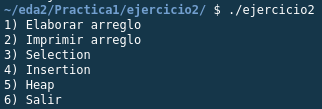
\includegraphics[scale = 0.8]{images/e2-main}
			\caption{Menu principal}
		\end{figure}
	
		Al momento de seleccionar cualquier opción, el programa utiliza la función \emph{switch()} para ejecutar el código indicado por el usuario.
		
			\subsubsection{Opción 1: Elaborar arreglo}
			
			La primera opción que es la de elaborar arreglo, pide inicialmente el numero de elementos a elegir dado esto, utiliza la función \emph{realloc()} para crear espacio en el arreglo dinámico en función de los elementos requeridos por el usuario.
			
			Después entra en un \emph{for-loop} que itera desde \textbf{0} hasta \textbf{n - 1} veces el espacio demandado y en cada ciclo se genera un numero al azar con la función \emph{rand()} y la cual se obtiene el modulo entre 100, lo que nos proporciona los últimos dos dígitos del numero creado ya que \emph{rand()} genera enteros de 8 dígitos
			
			Cada uno de estos números se acomoda de acuerdo a al indice del contador \textbf{i} en el arreglo dinámico
			
			\begin{figure}[h]
				\centering
				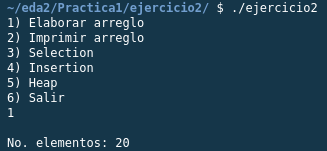
\includegraphics[scale = 0.8]{images/e2-1}
				\caption{Seleccionando opción 1 e ingresando numero de elementos deseados.}
			\end{figure}
		
			\subsubsection{Opción 2: Imprimir arreglo}
			
			La opción 2 simplemente imprime el arreglo que se acaba de crear. Utiliza un \emph{for-loop} para que de igual manera corre desde \textbf{0} hasta \textbf{n - 1} y simplemente utiliza la función \emph{printf()} dentro de cada iteración para mostrar en pantalla cada elemento dentro de la variable \textbf{arr}.
			
			\begin{figure}[H]
				\centering
				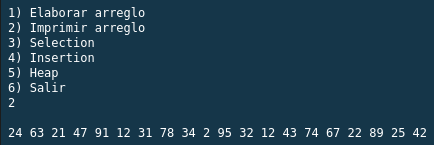
\includegraphics[scale = 0.8]{images/e2-2}
				\caption{Arreglo impreso después de seleccionar opción 2}
			\end{figure}
			
			\subsubsection{Opción 3: Selection Sort}
			
			Esta opción ejecuta la función \emph{selectionSort()} de la biblioteca \verb*|ordenamientos.c|. Al momento de ejecutarla toma como argumentos el arreglo dinámico creado \textbf{arr} así como la variable \textbf{n} que contiene el valor de la cantidad de elementos dentro del arreglo.
			
			La función itera \textbf{n - 1} veces hasta ordenar el arreglo que originalmente se encontraba en desorden.
			
			\begin{figure}[H]
				\centering
				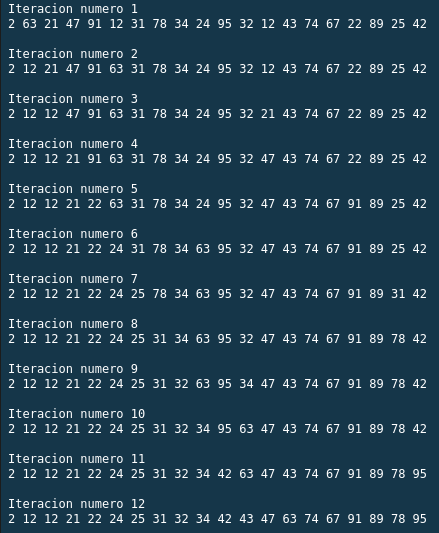
\includegraphics[scale = 0.8]{images/e2-3-1}
				\caption{Se muestra como se modifica el arreglo en los primeros 12 ciclos.}
			\end{figure}
		
			\begin{figure}[H]
				\centering
				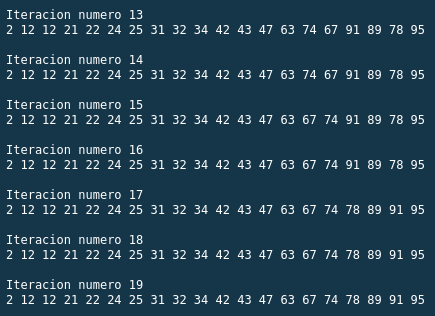
\includegraphics[scale = 0.8]{images/e2-3-2}
				\caption{Se muestra como se modifica el arreglo en últimos ciclos.}
			\end{figure}
			\newpage
			
			\subsubsection{Opcion 4: Insertion Sort}
			
			La opción numero 4 corresponde al \emph{insertionSort()} que al igual que el \emph{selectionSort} usa una de las funciones alojadas en la biblioteca \verb*|utilidades.h| para imprimir en pantalla cada una de las modificaciones del arreglo que se pretende ordenar.
			
			Modificamos el arreglo pasado para crear uno nuevo con la misma cantidad de elementos que el anterior y poder visualizar los ciclos de \emph{selectionSort} que de igual forma corre desde \textbf{0} hasta \textbf{n - 1} iteraciones por lo cual nos da de igual forma 20 arreglos impresos.
			
			\begin{figure}[H]
				\centering
				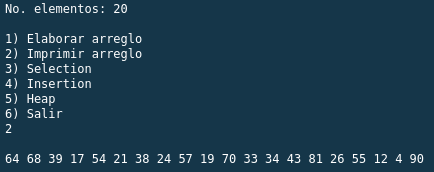
\includegraphics[scale = 0.8]{images/e2-4-1}
				\caption{Creando nuevo arreglo e imprimiendo sus valores}
			\end{figure}
			\newpage
		
			Después de esto, procedemos a seleccionar la opción 4 y nos muestra el programa como se va modificando el arreglo en cada ciclo del algoritmo.
			
			\begin{figure}[H]
				\centering
				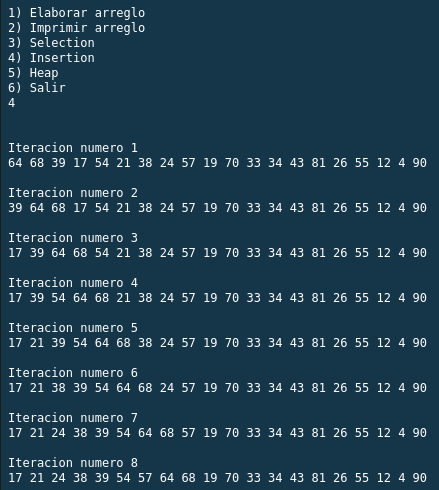
\includegraphics[scale = 0.8]{images/e2-4-2}
				\caption{Primeras 8 iteraciones de la opción 4}
			\end{figure}
		
			\begin{figure}[H]
				\centering
				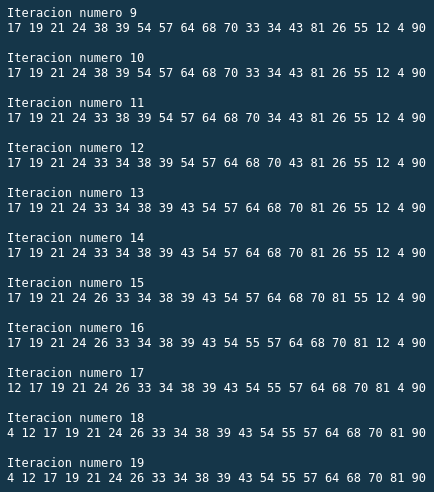
\includegraphics[scale = 0.8]{images/e2-4-3}
				\caption{Ultimas 11 iteraciones de la opción 4}
			\end{figure}
			\newpage
		
			\subsubsection{Opcion 5: Heap Sort}
			
			Repetimos la misma dinámica que con la opción 4, creamos un nuevo arreglo para apreciar el funcionamiento de \emph{heapSort()} y acto seguido procedemos a correr el algoritmo seleccionando la opción 5 de el programa.
			
			Se puede como el algoritmo hace uso primeramente de la función \emph{buildHeap} y una vez terminado comienza a remover la raíz del HEAP hasta que el arreglo queda completamente ordenado.
			
			\begin{figure}[H]
				\centering
				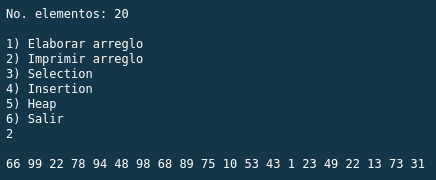
\includegraphics[scale = 0.8]{images/e2-5-1}
				\caption{Creando nuevo arreglo para HeapSort}
			\end{figure}
			
			\begin{figure}[H]
				\centering
				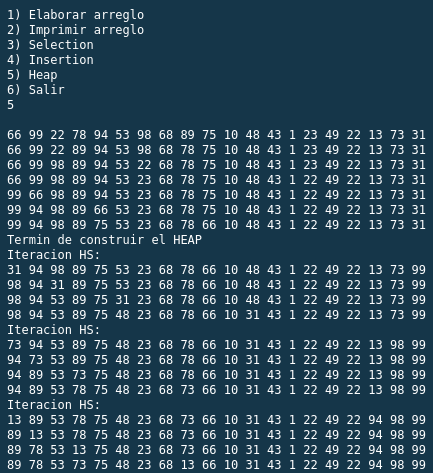
\includegraphics[scale = 0.8]{images/e2-5-2}
				\caption{Se crea el heap y después se comienza a remover las raíces}
			\end{figure}
			
			\begin{figure}[H]
				\centering
				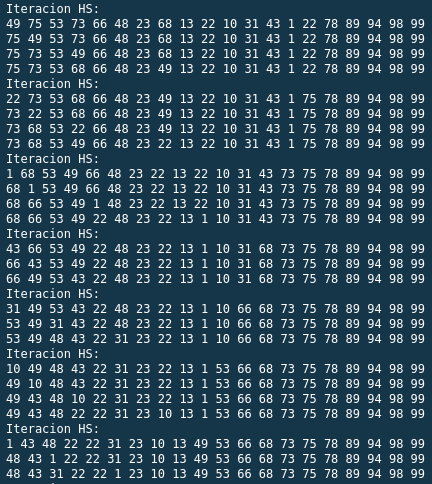
\includegraphics[scale = 0.8]{images/e2-5-3}
				\caption{Continua iterando el algoritmo}
			\end{figure}
		
			\begin{figure}[H]
				\centering
				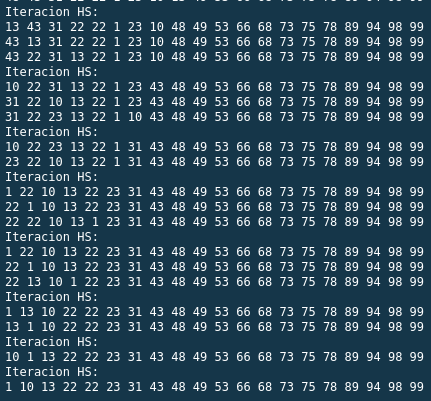
\includegraphics[scale = 0.8]{images/e2-5-4}
				\caption{Finaliza el algoritmo y se aprecia al final la lista ordenada ascendentemente}
			\end{figure}
			\newpage
		
			\subsubsection{Opcion 6: Salir}
			
			Para salir del programa, solo se escoge la opción 6 y automáticamente se rompen los ciclos y se finaliza el programa.
			
			\begin{figure}[H]
				\centering
				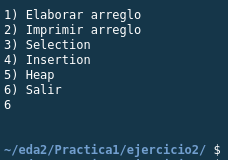
\includegraphics[scale = 0.8]{images/e2-exit}
				\caption{Finalización del programa}
			\end{figure}
		\newpage
		
		\subsection{Ejercicio 3}
		
		Para este ejercicio modifique el programa de tal forma que se automatizaron los tamaños de los arreglos de acuerdo a lo requerido por el ejercicio y se hicieron pruebas con 3 formas de arreglos distintas por cada uno de los algoritmos de ordenamientos.\\
		
		\noindent Se probaron 5 tamaños distintos de arreglos:
		
		\begin{itemize}
			\item 10
			\item 100
			\item 500
			\item 1000
			\item 2000
		\end{itemize} 
		
		\noindent Y se usaron 3 tipos de arreglos para cada uno de esos tamaños:
		
		\begin{itemize}
			\item Ascendente
			\item Descendente
			\item Aleatorio
		\end{itemize} 
	
		\noindent Se ejecutaron 45 pruebas en total y esta fue la tabla general de resultados:
				
		\begin{figure}[H]
			\centering
			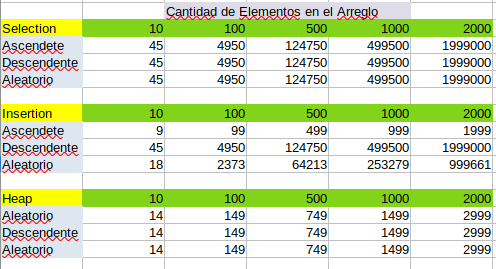
\includegraphics[scale = 0.8]{images/total - graph}
			\caption{Total de resultados}
		\end{figure}
	
			\subsubsection{Selection Sort:}
			
			Para el algoritmo de \emph{Selection Sort} se puede apreciar como debido a que su tiempo de complejidad es de $O(n^2)$ para todos los casos, los puntos de la grafica son constantes independientemente del tamaño del arreglo o de la forma en que se encuentre arreglado. De hecho en la grafica no se alcanza a apreciar los puntos rojos y amarillos puesto que son los mismos que los azules.
			
			\begin{figure}[H]
				\centering
				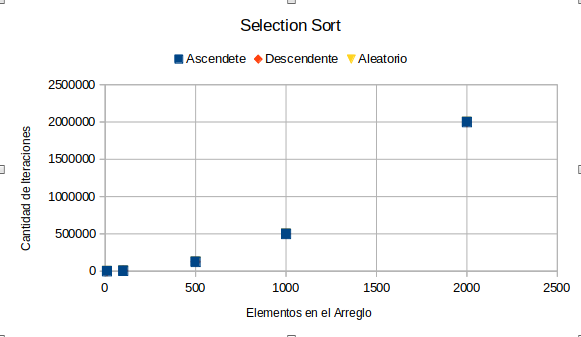
\includegraphics[scale = 0.65]{images/selection-graph}
				\caption{Grafica de Selection Sort}
			\end{figure}
			\newpage
		
		
			\subsubsection{Insertion Sort:}
			
			El algoritmo de \emph{Insertion Sort} a diferencia del anterior, tiene 3 tipos diferentes de complejidad temporal dependiendo de la forma en la que los arreglos se encuentren ordenados.
			
			\noindent Estas serian:
			
			\begin{itemize}
				\item Para el peor caso: $O(n^2)$
				\item Para el caso promedio: $\Theta(n^2)$
				\item Para el mejor caso: $\Omega(n^2)$ 
			\end{itemize}
	
			Podemos notar que para el caso de las listas aleatorias, no necesariamente se cumple esto sino es mas un caso promedio, puesto que no están en orden descendente lo que implica que el algoritmo tendría que hacer iteraciones a través de toda la lista.
	
	
			\begin{figure}[H]
				\centering
				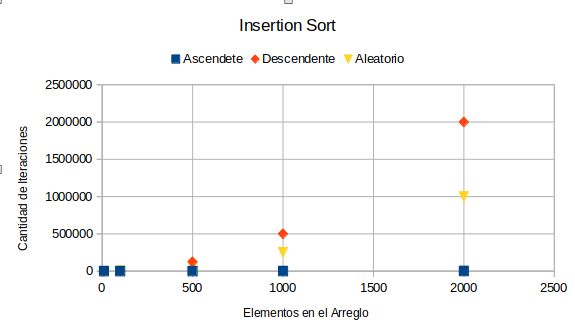
\includegraphics[scale = 0.65]{images/insertion- graph}
				\caption{Grafica de Insertion Sort}
			\end{figure}
			\newpage
			
				
			\subsubsection{Heap Sort:}
			
			Por ultimo, es notable como la grafica de \emph{Heap Sort} cumple con el tiempo logarítmico de $O(n log n)$ en la grafica que es casi una linea recta. Es un algoritmo que a pesar de no utilizar una estructura de datos lineal para ejecutarse, en realidad la forma en la que se ejecuta en el código es mas lineal de lo que parece, pues no usa muchos loops y su función principal \emph{Heapify} simplemente se reduce a hacer \emph{swaps} en el arreglo que utiliza que es lo que le ahorra mucho tiempo y memoria.

			\begin{figure}[H]
				\centering
				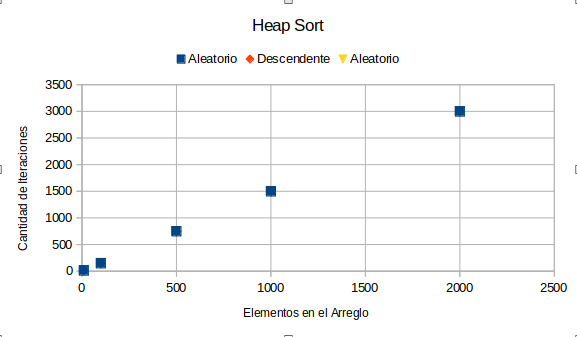
\includegraphics[scale = 0.6]{images/heap-graph}
				\caption{Grafica de Heap Sort}
			\end{figure}		
			\newpage
		
			\subsubsection{Capturas de Ejecucion}
			
			Aquí solo se incluyen las capturas de la ejecución del programa como lo pide el ejercicio.
			
			\begin{figure}[H]
				\begin{multicols}{2}
					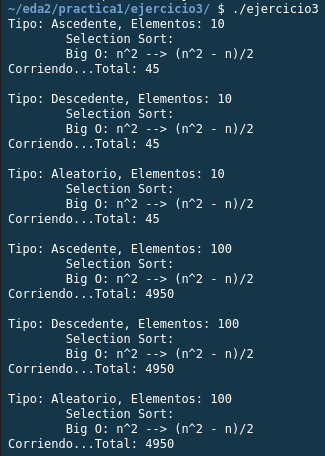
\includegraphics[width = \linewidth]{images/e3-1}\par
					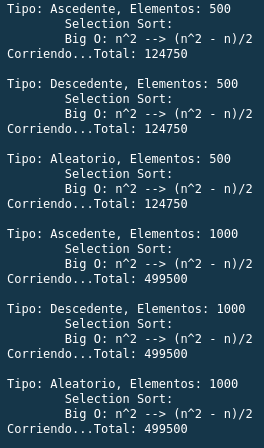
\includegraphics[width = \linewidth]{images/e3-2}\par
				\end{multicols}
			\caption{Output de programa automatizado}
			\end{figure}	
		
			\begin{figure}[H]
				\begin{multicols}{2}
					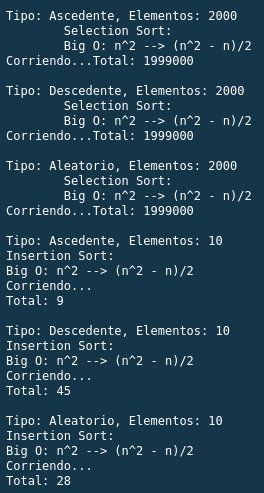
\includegraphics[width = \linewidth]{images/e3-3}\par
					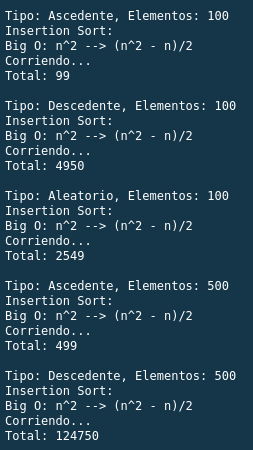
\includegraphics[width = \linewidth]{images/e3-4}\par
				\end{multicols}
			\caption{Output de programa automatizado}
			\end{figure}
		
			\begin{figure}[H]
				\begin{multicols}{2}
					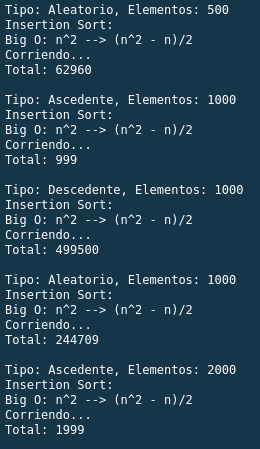
\includegraphics[width = \linewidth]{images/e3-5}\par
					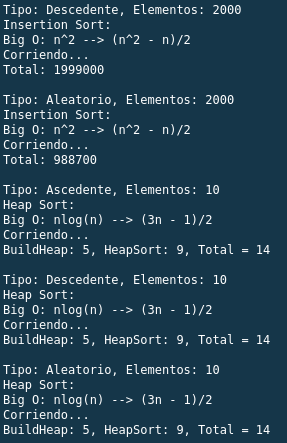
\includegraphics[width = \linewidth]{images/e3-6}\par
				\end{multicols}
				\caption{Output de programa automatizado}
			\end{figure}
		
			\begin{figure}[H]
				\begin{multicols}{2}
					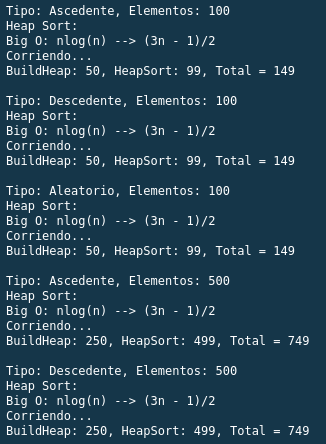
\includegraphics[width = \linewidth]{images/e3-8}\par
					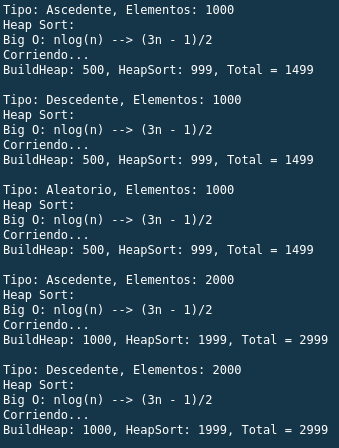
\includegraphics[width = \linewidth]{images/e3-9}\par
				\end{multicols}
				\caption{Output de programa automatizado}
			\end{figure}
		
			\begin{figure}[H]
				\centering
				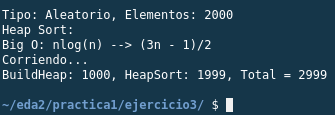
\includegraphics[scale = 0.8]{images/e3-10}
				\caption{Output de programa automatizado}
			\end{figure}
			
		\newpage
		
		\subsection{Ejercicio 4}
		
			\subsubsection{Ejecución OrdenamientoP1}
			
			\begin{figure}[H]
				\centering
				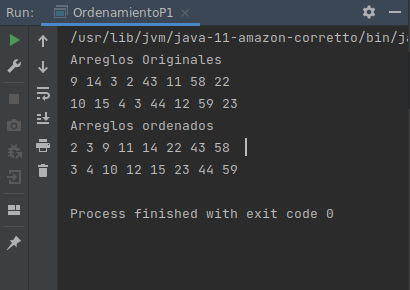
\includegraphics[scale = 0.6]{images/e4-1}
				\caption{Ejecución de OrdenamientoP1 en IntelliJIDE}
			\end{figure}
		
			\subsubsection{Revisión del Código}
			
			 Aun soy algo nuevo en esto de Java y sinceramente no entiendo muy bien como funciona el código que se encuentra en el programa, pero me recuerda mucho a los tipos de datos \emph{struct} que usamos en la clase de Estructura de Datos 1.\\
			
			Lo que veo en el archivo es que hay 3 archivos de clases y el archivo \\ \verb*|OrdenamientoP1.java| es el que contiene a la función \emph{main}, y un par de arreglos.\\
			
			Después la clase, imprime la leyenda \emph{Arreglos Originales} y después de esa linea, lo que noto es que el programa a través de \emph{Utilerias.imprimirArreglo()}, lo que hace es llamar al otro archivo donde se encuentra la clase \emph{Utilerias} y con un punto invoca a una funcion dentro de la clase que es la de \emph{imprimirArreglo()} la cual toma un argumento de un arreglo de números enteros y lo que veo es que al parecer en Java, se puede copiar un arreglo con un signo de \emph{=} como en \emph{Python}.\\
			
			De hecho es muy similar el programa a cuando en \emph{Python} se importan bibliotecas completas y para invocar sus funciones de usa el nombre de la biblioteca, seguido de un punto mas el nombre de la funcion que se desea ejecutar.\\
			
			Veo como de hecho los archivos-clases tienen distintos tipos de funciones dentro de si como por ejemplo, las clases de \emph{Inserción} y \emph{Selection} que contienen los algoritmos utilizados y que a su vez, de igual manera, invocan a las funciones incluidas en la clase \emph{Utilerias} que en ese caso es el método \emph{intercambiar()}.
			
			Por otro lado parece ser que al llamar al algoritmo de selección, lo que en realidad sucede es que se crea una nueva \textbf{instancia} de la clase \emph{Selection} que se llama igual, pero con minúscula al principio y a través de esta instancia se llama al algoritmo. Me imagino que esta instancia no se encuentra en el archivo de la clase como tal, sino ya en la memoria RAM de la computadora.\\
			
			Para finalizar se muestran los arreglos ordenados por medio del archivo-clase \emph{Utilerias} y el método \emph{imprimirArreglo()}.
		
		\newpage  
	
	\section{Conclusiones}
	
	Esta practica estuvo muy larga pero me gusto para ser la primera practica de la clase.\\ 
	
	Ya había dejado de trabajar con C y la practica afortunadamente me hizo recordar bastantes cosas que ya hace tiempo que no usaba y pude programar un poco, los algoritmos que usamos y experimentar con ellos.\\
	
	Los algoritmos me parecen interesantes, pero me gustaría indagar un poco mas en ellos, pues no creo que unicamente sirvan para ordenar números, sino que supongo que también deben de ser útiles cosas mas complejas como ordenar grandes cantidades de archivos, cadenas, palabras, etc. Me gustaría mas indagar en esa parte y saber como es que se utilizan en los programas que utilizamos a diario.\\
	
	El algoritmo de ordenamiento que mas me gusto fue \emph{HeapSort} porque se me hizo muy interesante este tipo de estructura no-lineal con la que trabaja y que adema es muy sencilla. Al principio me parecía que las estructuras de árbol, eran mas complicadas, pero entendiéndolas me di cuenta que la verdad son muy sencillas, inclusive podría decir que hasta mas sencillas que las demás estructuras de datos.\\
	
	De hecho, me di a la tarea de tratar de crear un algoritmo para imprimir los arreglos en forma de árbol y me quedo mas o menos así
	
	\begin{figure}[H]
		\centering
		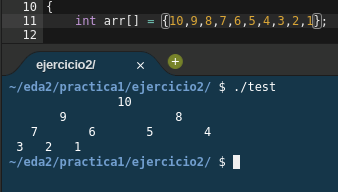
\includegraphics[scale = 0.8]{images/test}
		\caption{Impresión automática de arreglo en forma de árbol}
	\end{figure}
	
	La verdad es que mi algoritmo aun no es muy eficiente, pero me gusto experimentar con la forma de esa estructura.\\
	
	Otra cosa que me agrado bastante fue que este es el primer documento que hago en \LaTeX y aprendí mucho como usar el programa, mucha de la sintaxis del \emph{typeset}, insertar imágenes, formulas, accidentario, etc, ademas de que no sabia que también fue inventado por Donald Knut. (Quien fuera como el!)\\
	
	Por ultimo es la primera vez que experimento con \emph{Java}, pero creo que no me fue tan complicado ver como funciona la lógica del programa, creo que ya me va quedando claro que es un \textbf{objeto} y como se comportan. Recientemente adquirí el curso de Tim Buchalka para aprender a usarlo bien y es algo que he estado haciendo estos días Seguiré practicando para volverme mejor.\\
	
	Gracias por leer mi practica! 
	
\end{document}
